% =============================================================
% BODY (EN) – TEMPLATE WALKTHROUGH
% =============================================================

\section{Document Guide}
\vspace{2mm}

This document is designed as a modular project. The goal is to edit specific files (content and metadata) without touching the global layout.


\subsection{Project Structure}
\vspace{2mm}

\begin{itemize}
  \item \textbf{main-es.tex / main-en.tex}: entry points. They select the language and load \texttt{template.tex}.
  \item \textbf{template.tex}: global layout (cover, submission page, header/footer, packages).
  \item \textbf{metadata.tex}: assignment metadata (course, title, authors, instructor, date).
  \item \textbf{lang/es/body.tex}: Spanish content.
  \item \textbf{lang/en/body.tex}: English content (this file).
  \item \textbf{references.tex}: manual references at the end (no BibTeX).
  \item \textbf{assets/faculty-logo.png}: cover logo.
  \item \textbf{assets/figures/}: document figures.
\end{itemize}

\vspace{2mm}

\noindent
\textbf{Practical rule:} write content in \texttt{body.tex}. Edit assignment data in \texttt{metadata.tex}. Everything else is stable unless you want to change the global style.


\subsection{Build}
\vspace{2mm}

\begin{itemize}
  \item Build Spanish output: \texttt{main-es.tex}
  \item Build English output: \texttt{main-en.tex}
\end{itemize}

\vspace{2mm}

In VS Code (LaTeX Workshop), choose the corresponding main file and compile. The output PDF is generated according to your configured output directory (e.g., \texttt{out/latex/}).


\section{What To Edit}
\vspace{2mm}

\subsection{Metadata (course, title, authors, instructor)}
\vspace{2mm}

All metadata lives in \texttt{metadata.tex}:
\begin{itemize}
  \item Course (\texttt{\textbackslash subject})
  \item Assignment type (\texttt{\textbackslash doctype}) and ID (\texttt{\textbackslash docid})
  \item Title and subtitle (\texttt{\textbackslash titlee}, \texttt{\textbackslash subtitle})
  \item Authors (\texttt{\textbackslash authors}) and header short form (\texttt{\textbackslash authorsHeader})
  \item Instructor (\texttt{\textbackslash teacher}) and date (\texttt{\textbackslash placedate})
\end{itemize}

\vspace{2mm}

\subsection{Content}
\vspace{2mm}

Write the actual assignment (sections, solutions, conclusions) in \texttt{lang/en/body.tex}.


\section{Images And Figures}
\vspace{2mm}

Put figures in \texttt{assets/figures/}. Example:

\vspace{2mm}

\begin{center}
\begin{minipage}{0.92\textwidth}
\begin{lstlisting}
\begin{figure}[htbp]
  \centering
  \includegraphics[width=0.85\linewidth]{example-figure.png}
  \caption{Figure caption.}
\end{figure}
\end{lstlisting}
\end{minipage}
\end{center}

\vspace{2mm}

File names can be used without full paths when the image is in \texttt{assets/} or \texttt{assets/figures/} (already configured in the template).


\section{Programming Code}
\vspace{2mm}

Use \texttt{listings} for code blocks:

\vspace{2mm}

\begin{center}
\begin{minipage}{0.92\textwidth}
\begin{lstlisting}
\begin{lstlisting}
public class Main {
  public static void main(String[] args) {
    System.out.println("Hello, world!");
  }
}
\end{lstlisting}
\end{lstlisting}
\end{minipage}
\end{center}

\vspace{2mm}


\section{Diagrams And Logic Gates (TikZ)}
\vspace{2mm}

Minimal AND gate example:

\vspace{2mm}

\begin{center}
\begin{tikzpicture}[circuit logic US, scale=1.0, transform shape]
  \node[and gate, draw, logic gate inputs=nn] (G) at (0,0) {};
  \draw (-1.2,0.2) -- (G.input 1);
  \draw (-1.2,-0.2) -- (G.input 2);
  \draw (G.output) -- (1.2,0);
\end{tikzpicture}
\end{center}

\vspace{2mm}


\section{Plots (pgfplots)}
\vspace{2mm}

Minimal plot example:

\vspace{2mm}

\begin{center}
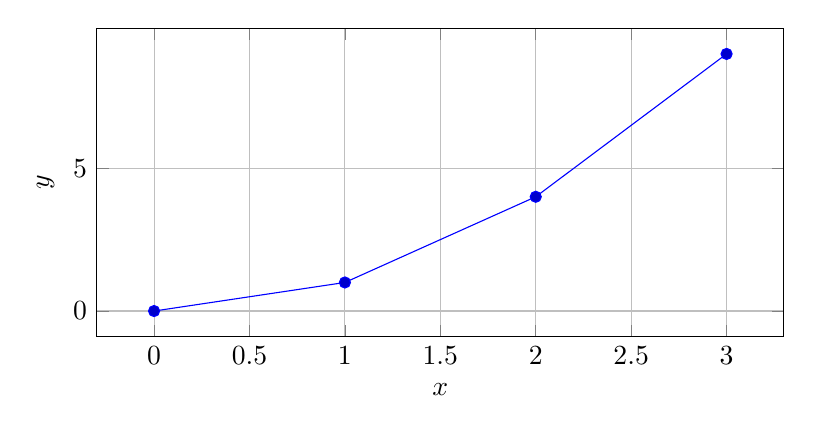
\begin{tikzpicture}
  \begin{axis}[
    width=0.85\linewidth,
    height=5.5cm,
    xlabel={$x$},
    ylabel={$y$},
    grid=major
  ]
    \addplot coordinates {(0,0) (1,1) (2,4) (3,9)};
  \end{axis}
\end{tikzpicture}
\end{center}

\vspace{2mm}


\section{References}
\vspace{2mm}

References are maintained in \texttt{references.tex} using \texttt{thebibliography} (manual, stable, no BibTeX).

\vspace{2mm}

\begin{center}
\begin{minipage}{0.92\textwidth}
\begin{lstlisting}
\begin{thebibliography}{9}

\bibitem{key}
Author, \textit{Title}. Publisher, Year.

\end{thebibliography}
\end{lstlisting}
\end{minipage}
\end{center}